\documentclass[]{article}
\usepackage[margin=2cm]{geometry}

%opening
\title{Exercises Set: Combinatorics\\ \large Solutions}
\author{DSBA Mathematics Refresher 2026}
\date{}

\usepackage{amsmath}
\usepackage{amsfonts}
\usepackage{amsthm}
\usepackage{amssymb}
\usepackage{mathrsfs}
\usepackage{stmaryrd}
\usepackage{tikz}

\newcommand{\Q}{\mathbb{Q}}
\newcommand{\N}{\mathbb{N}}
\newcommand{\Z}{\mathbb{Z}}
\newcommand{\R}{\mathbb{R}}
\newcommand{\Primes}{\mathbb{P}}
\newcommand{\st}{\text{ s.t. }}
\newcommand{\txtand}{\text{ and }}
\newcommand{\txtor}{\text{ or }}
\newcommand{\lxor}{\veebar}


\begin{document}

	\maketitle

	\section{Company employees (*)}

	Write $M$ for the set of men, $U$ for the set of union members and $W$ for the set of married employees ("wedded", to avoid a second $M$).
	The data is
	$$
	|M| = 300, \quad |U| = 352, \quad |W| = 424
	$$
	$$
	|U \cap M| = 188, \quad |W \cap M| = 166, \quad |U \cap W| = 208, \quad |U \cap W \cap M| = 144
	$$
	and the total number of employees is $800$.

	A \textit{single, non-union woman} is an employee who is in \textbf{none} of the three sets, so the answer is
	$$
	800 - |M \cup U \cup W|
	$$

	\paragraph{Method 1: inclusion-exclusion.}
	The formula for three sets is
	$$
	|M \cup U \cup W| = |M| + |U| + |W| - |U \cap M| - |W \cap M| - |U \cap W| + |U \cap W \cap M|
	$$
	Why this formula? Adding the three sets counts the employees belonging to exactly two of them twice, so we subtract the three pairwise intersections; but the employees belonging to all three, counted $3$ times and then removed $3$ times, have disappeared altogether, so we add them back once.

	Numerically:
	$$
	|M \cup U \cup W| = 300 + 352 + 424 - 188 - 166 - 208 + 144 = 1076 - 562 + 144 = 658
	$$
	so the answer is
	$$
	800 - 658 = \boxed{142}
	$$

	\paragraph{Method 2: filling in a Venn diagram.}
	It is instructive (and safer) to compute every region, starting from the middle and working outwards.
	Each time, we subtract from a given group the parts of it that we have already placed.
	\begin{itemize}
		\item All three: $144$.
		\item Union men, \textit{not} married: $188 - 144 = 44$.
		\item Married men, \textit{not} in the union: $166 - 144 = 22$.
		\item Married union members, \textit{not} men: $208 - 144 = 64$.
		\item Men only: $300 - (144 + 44 + 22) = 90$.
		\item Union only: $352 - (144 + 44 + 64) = 100$.
		\item Married only: $424 - (144 + 22 + 64) = 194$.
	\end{itemize}

	\begin{center}
		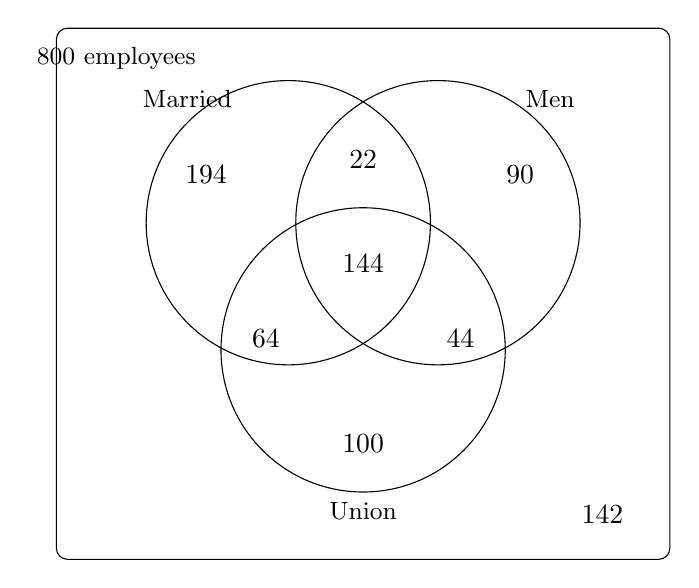
\begin{tikzpicture}[scale=0.95]
			\draw[rounded corners] (-4.1,-3.9) rectangle (4.1,3.2);
			\node at (-3.3,2.8) {\small $800$ employees};
			\draw (-1,0.6) circle (1.9);
			\draw (1,0.6) circle (1.9);
			\draw (0,-1.1) circle (1.9);
			\node at (-2.35,2.25) {\small Married};
			\node at (2.5,2.25) {\small Men};
			\node at (0,-3.25) {\small Union};
			% regions
			\node at (-2.1,1.25) {$194$};
			\node at (2.1,1.25) {$90$};
			\node at (0,-2.35) {$100$};
			\node at (0,1.45) {$22$};
			\node at (-1.3,-0.95) {$64$};
			\node at (1.3,-0.95) {$44$};
			\node at (0,0.05) {$144$};
			\node at (3.2,-3.3) {$142$};
		\end{tikzpicture}
	\end{center}

	The seven regions add up to
	$$
	144 + 44 + 22 + 64 + 90 + 100 + 194 = 658
	$$
	and therefore
	$$
	800 - 658 = 142
	$$

	\textbf{There are $142$ single women who are not in the union.}


	\section{The padlock}

	The code is an ordered sequence of $4$ digits, each from $0$ to $9$, and digits may be repeated unless stated otherwise.
	Every question below is solved with the \textbf{multiplication principle}: if a choice is made in successive independent steps, the number of possibilities is the product of the number of possibilities at each step.

	\paragraph{1. How many possible codes?}
	There are $10$ possibilities for each of the $4$ digits:
	$$
	10 \times 10 \times 10 \times 10 = 10^4 = \boxed{10\,000}
	$$

	\paragraph{2. Codes with 4 different digits.}
	Now each digit used is no longer available for the following positions:
	\begin{center}
		\begin{tabular}{ll}
			$1^{\text{st}}$ digit: & $10$ possibilities \\
			$2^{\text{nd}}$ digit: & $9$ possibilities (all but the first) \\
			$3^{\text{rd}}$ digit: & $8$ possibilities \\
			$4^{\text{th}}$ digit: & $7$ possibilities
		\end{tabular}
	\end{center}
	$$
	10 \times 9 \times 8 \times 7 = \frac{10!}{6!} = \boxed{5\,040}
	$$
	This is the number of \textbf{arrangements} (ordered selections without repetition) of $4$ digits among $10$.

	\paragraph{3. Codes ending with an even number.}
	The last digit must be one of $0, 2, 4, 6, 8$, so $5$ possibilities, and the first three are free:
	$$
	10 \times 10 \times 10 \times 5 = \boxed{5\,000}
	$$
	which is indeed half of the total: exactly one code out of two ends with an even digit.

	\paragraph{4. Codes ending with an even number, with 4 different digits.}
	Here the order of the choices matters for the \textit{counting} (not for the code): we start with the constrained position.
	\begin{center}
		\begin{tabular}{ll}
			$4^{\text{th}}$ digit: & $5$ possibilities (it must be even) \\
			$1^{\text{st}}$ digit: & $9$ possibilities (any digit but the last one) \\
			$2^{\text{nd}}$ digit: & $8$ possibilities \\
			$3^{\text{rd}}$ digit: & $7$ possibilities
		\end{tabular}
	\end{center}
	$$
	5 \times 9 \times 8 \times 7 = \boxed{2\,520}
	$$

	\textit{Remark:} had we started with the first digit, we would have been stuck --- the number of possibilities left for the last digit would depend on whether the digits already used were even or odd.
	\textbf{Always deal with the constrained positions first.}

	\paragraph{5. Codes containing at least one digit 4.}
	Counting these directly is painful (there may be one, two, three or four $4$'s, in any positions).
	It is much easier to count the \textbf{opposite}: the codes containing \textit{no} $4$ at all.
	For those, each of the $4$ positions has $9$ possibilities (every digit but $4$), so there are $9^4 = 6\,561$ of them, and
	$$
	\underbrace{10^4}_{\text{all codes}} - \underbrace{9^4}_{\text{without any } 4} = 10\,000 - 6\,561 = \boxed{3\,439}
	$$

	\textit{"At least one" is almost always a signal to count the complement.}

	\paragraph{6. Codes containing exactly one digit 4.}
	We choose where the $4$ goes, then fill the rest:
	\begin{itemize}
		\item $4$ possibilities for the position of the digit $4$;
		\item $9$ possibilities for each of the $3$ remaining positions (any digit but $4$, since we want \textit{exactly} one).
	\end{itemize}
	$$
	4 \times 9^3 = 4 \times 729 = \boxed{2\,916}
	$$

	\textit{Check:} $2\,916 < 3\,439$, as it must be --- "exactly one" is a particular case of "at least one".
	The difference, $523$, counts the codes with two, three or four $4$'s.


	\section{Airplanes Company}

	The $4$ airplanes are distinguishable, so we assign a crew to each of them in turn.

	\paragraph{The pilots.}
	Assigning $4$ distinct pilots to $4$ distinct airplanes is choosing an order for the pilots:
	$$
	4! = 24 \text{ ways}
	$$

	\paragraph{The flight attendants.}
	We must split $8$ flight attendants into $4$ pairs, one per airplane.
	Here, the order \textit{within} a pair does not matter (the two attendants of a plane are simply "the crew of that plane"), so we use \textbf{binomial coefficients}:
	$$
	\binom{n}{k} = \frac{n!}{k! \, (n-k)!}
	$$
	which counts the number of ways of choosing $k$ objects among $n$ \textit{without order}.
	\begin{center}
		\begin{tabular}{ll}
			$1^{\text{st}}$ airplane: & $\binom{8}{2} = 28$ ways (choose $2$ attendants among the $8$ available) \\[4pt]
			$2^{\text{nd}}$ airplane: & $\binom{6}{2} = 15$ ways \\[4pt]
			$3^{\text{rd}}$ airplane: & $\binom{4}{2} = 6$ ways \\[4pt]
			$4^{\text{th}}$ airplane: & $\binom{2}{2} = 1$ way (the two who are left)
		\end{tabular}
	\end{center}
	$$
	\binom{8}{2}\binom{6}{2}\binom{4}{2}\binom{2}{2} = 28 \times 15 \times 6 \times 1 = 2\,520 \text{ ways}
	$$

	\paragraph{Total.}
	The two choices are independent, so
	$$
	4! \times \binom{8}{2}\binom{6}{2}\binom{4}{2}\binom{2}{2} = 24 \times 2\,520 = \boxed{60\,480}
	$$

	\paragraph{Remark: why the binomial coefficient looks like that.}
	To choose $k$ objects among $n$ \textit{in order}, there are $n (n-1) \cdots (n-k+1) = \frac{n!}{(n-k)!}$ possibilities.
	But each unordered selection of $k$ objects has been counted once for each of its $k!$ orderings, so we divide by $k!$, which gives $\binom{n}{k} = \frac{n!}{k!(n-k)!}$.

	This also gives a quicker route to the $2\,520$ above: line up the $8$ attendants ($8!$ ways) and give the first two to plane $1$, the next two to plane $2$, and so on.
	Each assignment is obtained $2!$ times per airplane (the two members of a crew can be swapped), hence
	$$
	\frac{8!}{2! \, 2! \, 2! \, 2!} = \frac{40\,320}{16} = 2\,520 \ \checkmark
	$$


	\section{Bookshelf (*)}

	There are $4$ mathematics books, $6$ physics books and $3$ chemistry books, all distinct: $13$ books in total.

	\paragraph{If the books are grouped by subject.}
	Two independent things have to be decided:
	\begin{itemize}
		\item the order of the three \textit{groups} on the shelf: $3! = 6$ ways;
		\item the order of the books \textit{inside} each group: $4!$ for mathematics, $6!$ for physics, $3!$ for chemistry.
	\end{itemize}
	$$
	3! \times 4! \times 6! \times 3! = 6 \times 24 \times 720 \times 6 = \boxed{622\,080}
	$$

	\paragraph{If only the mathematics books are grouped.}
	The trick is to treat the mathematics block as a \textbf{single object}.
	We then have to order
	$$
	\underbrace{1}_{\text{the maths block}} + \underbrace{6}_{\text{physics}} + \underbrace{3}_{\text{chemistry}} = 10 \text{ objects}
	$$
	which can be done in $10!$ ways; and inside the block, the $4$ mathematics books can be ordered in $4!$ ways:
	$$
	4! \times 10! = 24 \times 3\,628\,800 = \boxed{87\,091\,200}
	$$

	\textit{Check:} this is much larger than the previous answer, which is reassuring --- the second situation is far less constrained than the first.


	\section{ESSEC's Stairs (*)}

	Let $F(n)$ be the number of ways of climbing a staircase of $n$ steps, going up either $1$ or $2$ steps at a time.
	Let us compute the first values by hand:
	$$
	\begin{array}{c|c|l}
		n & F(n) & \text{the different climbs} \\
		\hline
		0 & 1 & \text{do nothing} \\
		1 & 1 & 1 \\
		2 & 2 & 1+1 \ ; \ 2 \\
		3 & 3 & 1+1+1 \ ; \ 2+1 \ ; \ 1+2 \\
		4 & 5 & 1+1+1+1 \ ; \ 2+1+1 \ ; \ 1+2+1 \ ; \ 1+1+2 \ ; \ 2+2 \\
		5 & 8 & \dots \\
		6 & 13 & \dots
	\end{array}
	$$
	These are the Fibonacci numbers --- but \textit{why}?

	\paragraph{The recurrence.}
	Consider any way of climbing $n$ steps, and look only at \textbf{the first move}.
	There are two possibilities, and they exclude each other:
	\begin{itemize}
		\item the first move is a single step; there remain $n-1$ steps to climb, in $F(n-1)$ ways;
		\item the first move is a double step; there remain $n-2$ steps to climb, in $F(n-2)$ ways.
	\end{itemize}
	Every climb falls into exactly one of these two cases, so we may add the two counts:
	$$
	F(n) = F(n-1) + F(n-2), \qquad \text{with } F(0) = 1 \text{ and } F(1) = 1
	$$
	\begin{center}
		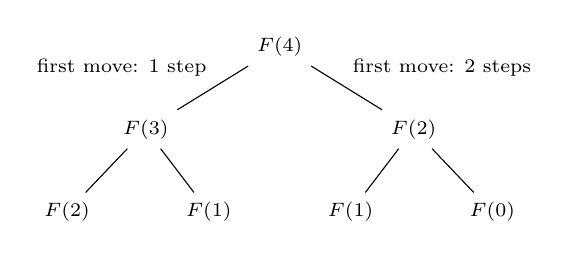
\begin{tikzpicture}[scale=1.0,every node/.style={font=\scriptsize}]
			\node (r) at (0,2.1) {$F(4)$};
			\node (a) at (-1.7,1.05) {$F(3)$};
			\node (b) at (1.7,1.05) {$F(2)$};
			\node (a1) at (-2.7,0) {$F(2)$};
			\node (a2) at (-0.9,0) {$F(1)$};
			\node (b1) at (0.9,0) {$F(1)$};
			\node (b2) at (2.7,0) {$F(0)$};
			\draw (r) -- node[above left,pos=0.45] {first move: $1$ step} (a);
			\draw (r) -- node[above right,pos=0.45] {first move: $2$ steps} (b);
			\draw (a) -- (a1); \draw (a) -- (a2);
			\draw (b) -- (b1); \draw (b) -- (b2);
		\end{tikzpicture}
	\end{center}
	Each climb is sorted into exactly one of the two branches according to its first move, and the same
	question then reappears on a shorter staircase --- which is what makes the count recursive.

	This is precisely the Fibonacci sequence.

	\paragraph{The answer.}
	We now only have to iterate up to $n = 16$:
	$$
	\begin{array}{c|ccccccccccccccccc}
		n & 0 & 1 & 2 & 3 & 4 & 5 & 6 & 7 & 8 & 9 & 10 & 11 & 12 & 13 & 14 & 15 & 16 \\
		\hline
		F(n) & 1 & 1 & 2 & 3 & 5 & 8 & 13 & 21 & 34 & 55 & 89 & 144 & 233 & 377 & 610 & 987 & 1597
	\end{array}
	$$
	$$
	F(16) = \boxed{1\,597}
	$$

	\textit{Remark:} note how the "first move" argument replaced a hopeless enumeration by two smaller versions of the same problem.
	Splitting a count into exclusive cases (here, by conditioning on the first move) is one of the most useful techniques in combinatorics.

\end{document}
